\section{Model}
\label{sec:model}

\setlength{\tabcolsep}{2pt}
\begin{figure*}
\begin{center}
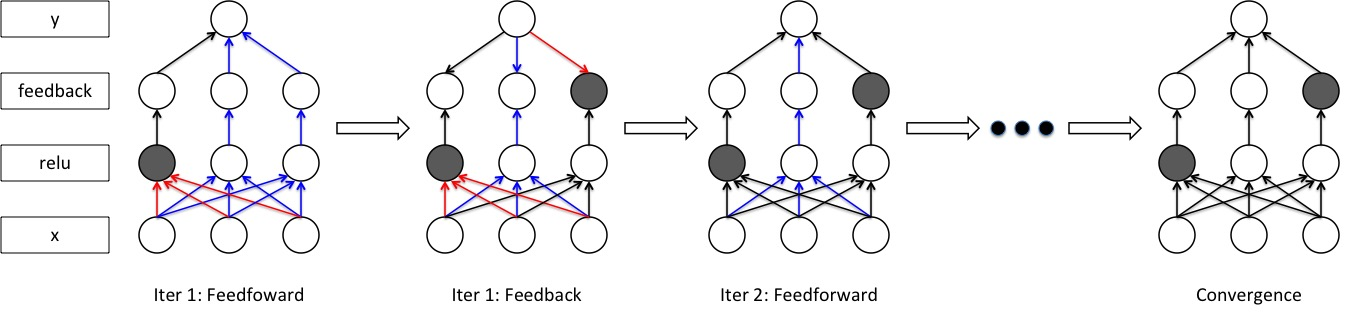
\includegraphics[width=0.95\linewidth]{figs/model/model}
% \vspace{-10pt}
\caption{Illustration of our feedback model and its inference process. At the first iteration, the model performs as a feedforward neural net. Then given the top signal neuron, the hidden layers update their gates to maximize the confidence for the top neuron. This process continues until convergence.}
\label{fig:visual_compare}
% \vspace{-30pt}
\end{center}
\end{figure*}

\subsection{Updating Hidden Layer Activations}
Our work is inspired by~\cite{xxx} where they design a ConvNet visualization technique as looking for an $L_2$ regularised image such that the class score $S_c$ is maximized. The procedure is related to the ConvNet training procedure, where the back-propagation is used to optimise the layer weights. The optimisation is performed with respect to the input image, while the weights are fixed to those found during the training stage.

Given an image $I_0$ and a pre-trained feedforward neural network with learned parameters $w$, we optimize the neuron activiations $h$ over all the hidden layers to maximize the class score output:
\begin{equation}
\begin{aligned}
  \max_h S_c(I_0, h) \\
  s.t.\ h_i \in \{0, 1\}
\end{aligned}
\end{equation}

This leads to an integer programming, which is a NP-hard problem given the current deep convolutional neural net structure. To obtain a good solution, we conduct two ways to optimize it: the layer-wise coordinate descent method and linear relaxation.

In the linear relaxation, we rephrase the problem as:
\begin{equation}
\begin{aligned}
  \max_h S_c(I_0, h) \\
  s.t.\ 0 \leq h_i \leq 1
\end{aligned}
\end{equation}

We use the backpropagation algorithm and gradient descent to optimize $h$. After convergence we discretize $h$ to 0 or 1.

We model the top down as another type of activation variable, similar as ReLu. However, this unit activates based on the the overall information of bottom-up responses and top-down messages. 

In practice, we treat the inference process as discriminatively optimize the final class node. 

Optimizing such function results in an integer programming, if we treat h as binary variables. 

During optimization, we proposed two ways to deal with it, 1. coordinate descent 2. continuous relaxation

Hard optimization: The coordinate descent frameworks stand in this way: 1. Initialize h as all 1 meaning the gate is open, compute feedfoward messages to the class node, then given the current activation status, optimize the last layer h to maximize the class output, given the updates last layer h, keep optimizing lower layers. And reiterate this process.

Soft optimization: The continuous relaxation falls in below way, compute the gradient of class node y given h, use gradient descent update h, and keep until this until convergence.

\subsection{Relationship to Deconvolutional Neural Networks}

Following this, deconvnet can be viewed as a one iteration of our hard optimization

\subsection{Implementation Details}
